%
% filterarten.tex -- Bild zum Thema Optische Fouriertransformation <opt>
%
% (c) 2023 Marco Niederberger, Yanick Schoch; OST Ostschweizer Fachhochschule
%

\documentclass[tikz]{standalone}
\def\skala{1}

%% Create a filter with a custom image on top
%% %1: Position in x direction
%% %2: Text below figure
%% %3: Actual code to draw the filter
\newcommand{\filterBackground}[3]{%
        #3 % Custom per each filter
        \draw[draw=none](#1, 0) circle (1.6); %Make drawing symmetric

        % x and y axis
        \draw[->, dashed] (-1.4+#1,0)--(1.4+#1,0) node[right, above]{$\omega_x$};
        \draw[->, dashed] (#1,-1.4)--(#1,1.4) node[right]{$\omega_y$};

        \node[draw=none] at (#1, -2) {#2};
}

\def\posLowpass{-5.4}
\def\posHighpass{-1.8}
\def\posBandpass{-\posHighpass}
\def\posBandstop{-\posLowpass}

\def\sizeInfitite{1}

\begin{document}
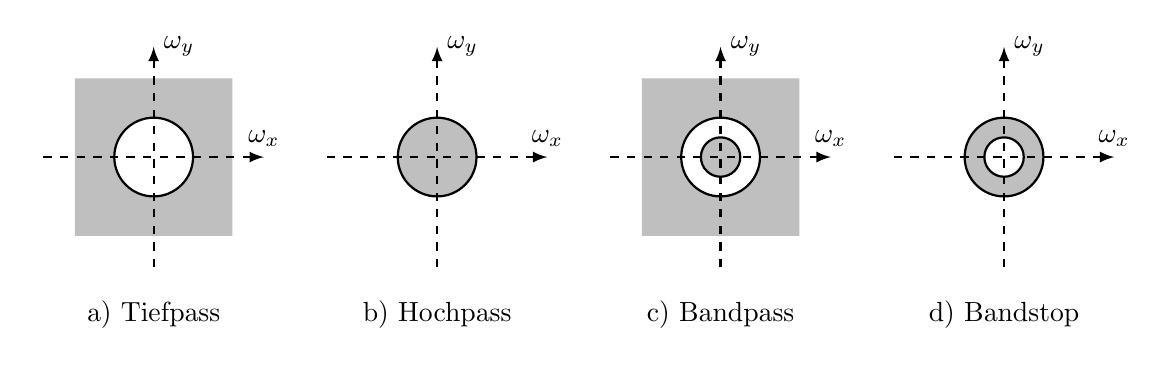
\begin{tikzpicture}[>=latex,thick,scale=\skala]
    % Lowpass
    \filterBackground{\posLowpass}{a) Tiefpass}{
        \draw[draw=none, fill=lightgray] (\posLowpass - \sizeInfitite,0 - \sizeInfitite) rectangle (\posLowpass + \sizeInfitite,0 + \sizeInfitite) (\posLowpass,0) circle (0.5);
        \draw[draw] (\posLowpass,0) circle (0.5);
        % \node[label={135:{$\omega_c$}}, circle, fill, inner sep=1pt] at (\posLowpass - 0.5, 0) {};
    }

    % Highpass
    \filterBackground{\posHighpass}{b) Hochpass}{
        \draw[draw,fill=lightgray,] (\posHighpass, 0) circle (0.5);
        % \node[label={135:{$\omega_c$}}, circle, fill, inner sep=1pt] at (\posHighpass - 0.5, 0) {};
    }

    % Bandpass
    \filterBackground{\posBandpass}{c) Bandpass}{
        \draw[draw=none, fill=lightgray] (\posBandpass - \sizeInfitite,0 - \sizeInfitite) rectangle (\posBandpass + \sizeInfitite,0 + \sizeInfitite) (\posBandpass,0) circle (0.5);
        \draw[draw] (\posBandpass, 0) circle (0.5);
        \draw[draw, fill = lightgray] (\posBandpass, 0) circle (0.25);
    }

    % Bandstop
    \filterBackground{\posBandstop}{d) Bandstop}{
        \path [draw,fill=lightgray, even odd rule] (\posBandstop, 0) circle (0.5) (\posBandstop, 0) circle (0.25);
    }
\end{tikzpicture}
\end{document}
